% Also note that the "draftcls" or "draftclsnofoot", not "draft", option
% should be used if it is desired that the figures are to be displayed in
% draft mode.
%
%\documentclass[journal]{IEEEtran}
\documentclass[final,peerreview,onecolumn]{IEEEtran}
% ***PACKAGES ***
%
\usepackage{cite}
\usepackage[pdftex]{graphicx}
\usepackage{epstopdf}
%\usepackage{graphicx}
 % declare the path(s) where your graphic files are
\graphicspath{{./images/}}
  % and their extensions so you won't have to specify these with
  % every instance of \includegraphics
\DeclareGraphicsExtensions{.pdf,.png,.eps}


% *** MATH PACKAGES ***

\usepackage[cmex10]{amsmath}
\interdisplaylinepenalty=2500
% *** ALIGNMENT PACKAGES ***
%
\usepackage{array}
\usepackage{mdwmath}
\usepackage{mdwtab}
\usepackage{eqparbox}


% *** SUBFIGURE PACKAGES ***
\usepackage[tight,footnotesize]{subfigure}
% subfigure.sty was written by Steven Douglas Cochran. This package makes it
% easy to put subfigures in your figures. e.g., "Figure 1a and 1b". For IEEE
% work, it is a good idea to load it with the tight package option to reduce
% the amount of white space around the subfigures. subfigure.sty is already
% installed on most LaTeX systems. The latest version and documentation can
% be obtained at:
% http://www.ctan.org/tex-archive/obsolete/macros/latex/contrib/subfigure/
% subfigure.sty has been superceeded by subfig.sty.

%\usepackage[caption=false]{caption}
%\usepackage[font=footnotesize]{subfig}
% subfig.sty, also written by Steven Douglas Cochran, is the modern
% replacement for subfigure.sty. However, subfig.sty requires and
% automatically loads Axel Sommerfeldt's caption.sty which will override
% IEEEtran.cls handling of captions and this will result in nonIEEE style
% figure/table captions. To prevent this problem, be sure and preload
% caption.sty with its "caption=false" package option. This is will preserve
% IEEEtran.cls handing of captions. Version 1.3 (2005/06/28) and later
% (recommended due to many improvements over 1.2) of subfig.sty supports
% the caption=false option directly:
%\usepackage[caption=false,font=footnotesize]{subfig}
%
% The latest version and documentation can be obtained at:
% http://www.ctan.org/tex-archive/macros/latex/contrib/subfig/
% The latest version and documentation of caption.sty can be obtained at:
% http://www.ctan.org/tex-archive/macros/latex/contrib/caption/


% *** FLOAT PACKAGES ***
%
%\usepackage{fixltx2e}
% fixltx2e, the successor to the earlier fix2col.sty, was written by
% Frank Mittelbach and David Carlisle. This package corrects a few problems
% in the LaTeX2e kernel, the most notable of which is that in current
% LaTeX2e releases, the ordering of single and double column floats is not
% guaranteed to be preserved. Thus, an unpatched LaTeX2e can allow a
% single column figure to be placed prior to an earlier double column
% figure. The latest version and documentation can be found at:
% http://www.ctan.org/tex-archive/macros/latex/base/


%\usepackage{stfloats}
% stfloats.sty was written by Sigitas Tolusis. This package gives LaTeX2e
% the ability to do double column floats at the bottom of the page as well
% as the top. (e.g., "\begin{figure*}[!b]" is not normally possible in
% LaTeX2e). It also provides a command:
%\fnbelowfloat
% to enable the placement of footnotes below bottom floats (the standard
% LaTeX2e kernel puts them above bottom floats). This is an invasive package
% which rewrites many portions of the LaTeX2e float routines. It may not work
% with other packages that modify the LaTeX2e float routines. The latest
% version and documentation can be obtained at:
% http://www.ctan.org/tex-archive/macros/latex/contrib/sttools/
% Documentation is contained in the stfloats.sty comments as well as in the
% presfull.pdf file. Do not use the stfloats baselinefloat ability as IEEE
% does not allow \baselineskip to stretch. Authors submitting work to the
% IEEE should note that IEEE rarely uses double column equations and
% that authors should try to avoid such use. Do not be tempted to use the
% cuted.sty or midfloat.sty packages (also by Sigitas Tolusis) as IEEE does
% not format its papers in such ways.



% *** PDF, URL AND HYPERLINK PACKAGES ***
%
%\usepackage{url}
% url.sty was written by Donald Arseneau. It provides better support for
% handling and breaking URLs. url.sty is already installed on most LaTeX
% systems. The latest version can be obtained at:
% http://www.ctan.org/tex-archive/macros/latex/contrib/misc/
% Read the url.sty source comments for usage information. Basically,
% \url{my_url_here}.

% correct bad hyphenation here
\hyphenation{op-tical net-works semi-conduc-tor}

\begin{document}
\setcounter{page}{1}

%
% paper title
% can use linebreaks \\ within to get better formatting as desired
\title{A Homopolar HTSG Topology for Large Direct Drive Wind Turbines}
 
 
 \author{Ozan~Keysan,~
         Markus~Mueller% <-this % stops a space

\thanks{O. Keysan and M.Mueller are with Institute for Energy Systems,
University of Edinburgh, Edinburgh, EH9 3JL U.K.
e-mail:o.keysan@ed.ac.uk, markus.mueller@ed.ac.uk}% <-this % stops a space
\thanks{Manuscript received April 19, 2005; revised January 11, 2007.}}
%\author{\IEEEauthorblockN{Ozan Keysan\IEEEauthorrefmark{1},
%Markus Mueller\IEEEauthorrefmark{2}}
%\IEEEauthorblockA{\IEEEauthorrefmark{1}\IEEEauthorrefmark{2}School of Engineering, Institute for Energy Systems\\
%University of Edinburgh,
%King's Buildings, Edinburgh EH9 3JL United Kingdom}
%\IEEEauthorblockA{\IEEEauthorrefmark{1}Email: o.keysan@ed.ac.uk}}
%Email: homer@thesimpsons.com}
%\IEEEauthorblockA{\IEEEauthorrefmark{3}Starfleet Academy, San Francisco, California 96678-2391\\
%Telephone: (800) 555--1212, Fax: (888) 555--1212}
%\IEEEauthorblockA{\IEEEauthorrefmark{4}Tyrell Inc., 123 Replicant Street, Los Angeles, California 90210--4321}}

%\maketitle
\IEEEpeerreviewmaketitle

\begin{abstract}

For offshore wind energy, there is a trend  towards larger wind turbines. The increased power take-off system mass increases the installation cost of the turbine. Direct-drive superconducting generators have the potential to reduce the installation cost of wind turbines. For a successful entry to offshore wind energy market, a HTS generator should be as reliable as conventional generators. It is proposed that a stationary superconducting dc-field winding may increase the reliability of the generator. An axial-flux homopolar generator topology is proposed to be used in low-speed high-torque applications. The topology is modified by using two superconducting field windings to obtain a bipolar flux density distribution for higher power density. Different core types and dimensions were examined to find the most suitable design and a conceptual design of 6 MW, 12 rpm generator is presented.


\end{abstract}


% Note that keywords are not normally used for peerreview papers.
%\begin{IEEEkeywords}
%IEEEtran, journal, \LaTeX, paper, template.
%\end{IEEEkeywords}


\section{Introduction}
\IEEEPARstart{T}{here} has been a remarkable increase in the installed renewable power capacity around the world for the last decade and this increase is expected to continue for many years \cite{Tong2010}. The onshore wind energy market is now quite mature, but there is a lot of ongoing research into offshore renewable energy devices which will benefit from higher wind speeds and higher capacity factors \cite{Tong2010}.  In offshore wind turbines, there is a trend towards higher power rated turbines to reduce installation and maintenance costs per kWh \cite{Bang2008}. According to market projections of \cite{offshore_wind_report2009}, annual world production of offshore wind turbines will continue to increase. Furthermore, the proportion of  the turbines rated over 5 MW will increase significantly for the next decade as seen from Fig. \ref{world_production}.

\begin{figure}[!h]
\centering
\includegraphics[width=3in]{world_turbine_production}
\caption{Emerging market projection for offshore wind energy converters (Data from \cite{offshore_wind_report2009}).}
\label{world_production}
\end{figure}


Currently, geared asynchronous machines hold a 70\% share of wind turbine generators \cite{Lesser2009}. Lesser \textit{et al.} compared costs of different generator types in \cite{Lesser2009}. They proposed that the aim of the offshore wind turbine industry is to manufacture 10 MW  turbines which cost \$ 2.7 M/MW or less. The current cost of wind turbines is about \$ 2 M/MW for onshore turbines and \$ 3.7 M/MW for offshore wind turbines with a typical rating of 2.5 MW for onshore and 3.6 MW for offshore \cite{Lesser2009}.

The feasible limit for an industrial 3-stage wind turbine gearbox is about 5 MW due to high torque requirements at very low speeds \cite{Lesser2009}. Moreover, gearboxes cause reliability issues in wind turbines. The reliability of wind turbine sub-assemblies have been compared in \cite{Spinato2009} using the data obtained from 6000 onshore wind turbines over 11 years. This study shows that, although the gearbox doesn't have the highest failure rate, the failures related to gearboxes result in the highest down-time periods (average 340 hours per failure). Note that, this data was obtained from onshore turbines; the downtime related to a gearbox failure for offshore turbines will be much higher, adding an extra cost of down-time on top of the maintenance cost. For example, the worst case scenario is a major failure at the beginning of the winter period and with no subsequent access to the turbine until the winter storms are gone \cite{Abrahamsen2010}.

There are some commercial solutions (mostly direct-drive permanent magnet generators) that aim to overcome this problem e.g. Harakosan, Vensys, Enercon. In \cite{Bang2008} different topologies for wind turbines have been compared. The highest power rated  commercial direct drive machine is the 4.5 MW, 13 rpm Enercon-E112 generator which has a 12 m diameter and 220 tonnes mass. The optimum weight for a 10 MW direct drive PM generator is greater than 300 metric tons including support structures with an air gap diameter greater than 10 meters \cite{Bang2008}. The installation cost of the turbine is directly related to the mass of the generator and nacelle. Moreover, the tower, the foundation and all other supporting structures have to be modified to carry the added mass of the generator. Considering the capability of current offshore installation vessels which is around 300 tonnes \cite{Lewis2007}, the demand for a high power density, low-speed direct-drive generator topology is clear.

One promising candidate to reduce the overall mass and volume of a large offshore wind turbine(up to 10 MW) power take-off system is High-Temperature Superconducting Generators (HTSG) \cite{Lesser2009, Lewis2007, Kalsi2004}. HTS machines can be scaled as fifth power of dimension in \cite{Kalsi2004} compared to third power for a conventional machine, which will become more dominant at direct-drive machines. It is stated in \cite{Lewis2007} that a 6 MW HTS direct drive generator may have 50 \% of the mass of a direct drive PM generator and the lower mass of generator may enable transport and installation of the turbine in one piece.

\begin{figure}[!t]
\centering
\includegraphics[width=3.5in]{generators_mass_comparison}
\caption{Mass of different large direct-drive machines as a function of the torque, bubble size represents the power rating.
EESM: Electrically excited synchronous machine, HTSG: High-temperature superconducting generator, PMG: Permanent-magnet generator. Dashed line represents generator mass to torque ratio ($m/T$) of 25 kg/kNm for permanent-magnet machines as given in \cite{Bang2008}. Continuous line is the linear trend line estimated using the HTS machines in the graph.}
\label{generators_mass_comparison}
\end{figure}

Data from direct-drive systems have been collected to compare mass to torque ratio of HTS machines with other type of generators. The result is presented in a bubble chart in Fig. \ref{generators_mass_comparison} and tabulated in Table \ref{generators_list}.  Note that, some of the machines are final designs or commercial products (e.g., Enercon, Harakosan), where some designs are provisional or it is not clear how the structural mass is estimated. Final designs tend to be heavier than initial designs, but it is believed that the graph will provide a good understanding of torque density capability of HTS machines.  The dashed line represents ratio of generator mass to torque for permanent-magnet machines which is estimated as 25 kg/kNm by Bang \textit{et al.} in \cite{Bang2008}. The Enercon-E112, which has a high $m/T$ ratio (66.6 kg/kNm) is the only copper field synchronous generator in the graph. The continuous line represents the linear trend line estimated using the HTS machines in the graph. The equation of the trend line is given in (\ref{mass_torque_eq}). It can be seen from the graph that HTS machines are generally lighter than PM generators for applications with torque requirements larger than 3000 kNm. There are two PMG topologies below the HTS machine trend line; a transversal flux permanent magnet machine \cite{Bang2009} and the NewGen topology which reduces the structural mass significantly \cite{Engstrom2004}. It should be noted that implementation of similar techniques to HTS machines can further decrease their mass. 

 \begin{equation}
     Mass(t)=0.011\times Torque(kNm)+45
     \label{mass_torque_eq}
 \end{equation}


\begin{table*}[t]
\caption{Comparison of generators torque density}
\label{generators_list}
\centering
\begin{tabular}{lllllll}
\hline
Manufacturer & Power & Speed & Mass & Torque & Mass/Torque & Type \\
 & (MW) & (RPM) & (tonnes) & (kNm) & (kg/kNm) & \\
\hline
\hline
AMSC \cite{Kalsi2006} & 36.5 & 120 & 75 & 2905 & 25.8 & HTSG \\
Converteam \cite{Lewis2007} & 8 & 12 & 100 & 6366 & 15.7 & HTSG  \\
Enercon-E112 \cite{Bang2008} & 4.5 & 13 & 220 & 3305 & 66.6 & EESM \\
Harakosan \cite{Duan2009}& 1.5 & 18 & 47.2 & 796 & 59.3 & PMG \\
Bang et. al. \cite{Bang2008} & 10 & 10 & 325 & 9543 & 34 & PMG (estimate)  \\
Lee et. al. \cite{Lee2008} & 5 & 230 & 18 & 207.6 & 86.7 &  HTSG(ASSM)  \\
 & 5 & 230 & 44 & 207.6 & 212 & HTSG(Homopolar)  \\
NewGen \cite{Engstrom2004} & 4 & 19 & 36.4 & 2010 & 18.1 & PMG  \\
Maki \cite{Maki2008} & 2 & 21.5 & 54 & 888 & 60.8 & HTSG  \\
 & 5 & 14.8 & 108 & 3226 & 33.5 & HTSG \\
 & 8 & 12 & 154 & 6366 & 24.2 & HTSG  \\
Abrahansen et. al. \cite{Abrahamsen2010}& 10 & 10.4 & 88 & 9182 & 9.6 & HTSG (economically infeasible)  \\
AMSC \cite{Snitchler2010} & 10 & 11 & 150 & 8681 & 17.3 & HTSG  \\
NREL-AMSC \cite{Maples2010} & 3.1 & 12.5 & 76 & 2368 & 32.1 & HTSG  \\
 & 6 & 12.3 & 97 & 4658 & 20.8 & HTSG  \\
 & 10 & 11.5 & 160 & 8303 & 19.3 & HTSG  \\
 & 3.1 & 12.5 & 90 & 2368 & 38 & PMG(not optimized)  \\
 & 6 & 12.3 & 177 & 4658 & 38 &  PMG(not optimized) \\
 & 10 & 11.5 & 315 & 8304 & 37.9 & PMG(4.3 m limited diameter)  \\
Bang et. al. \cite{Bang2009} & 5 & 12 & 90.8 & 3979 & 22.8 & TFPM  \\
 & 5 & 12 & 60.5 & 3979 & 15.2 & Ring-shaped TFPM  \\
The Switch \cite{Duan2009} & 3.8 & 21 & 81 & 1728 & 46.9 & PMG  \\
\hline
\end{tabular}
\end{table*}


%Ustu ayni texden aynen alinan cumleler var rewrite

\section{Double Sided Claw Pole Machine}

In \cite{} a radial flux claw pole machine is presented. The machine has a single stationary superconducting coil, which simplifies the cooling part.

In this design, the claw poles are rotated 90 degrees, and two axial claw poles are attaché together to operate as two independent machines as shown in…

Advantages:

The advantages of the double-sided claw pole topology can be summarised as:

\begin{itemize}
  \item Magnetic attraction forces on the large claw poles are symmetrical and cancel each other.
  \item Double armature winding configuration increases the modularity.
  \item SMC material is no longer required. All magnetic core sections can be manufactured using laminations.
  \item The superconducting coil back-core mass is reduced.
\end{itemize}



\section{Design of a 10 MW Superconducting Generator}

\subsection{Material Selection}

The proposed generator concept is iron cored, hence the power density of the machine is limited by the saturation of the magnetic core, which makes the material selection crucial. Vacuumschmelze manufactures a cobalt-iron alloy, which is called VacoFlux50, which  has an impressive magnetic saturation limit with 2.35 T at 16 kA/m \cite{vacoflux}. B-H characteristics of the VacoFlux50 is presented in \autoref{vacoflux-bh}.

Vacoflux50 is a very suitable material for superconducting machines with its high saturation limit.


\begin{figure}[t]
  \centering
    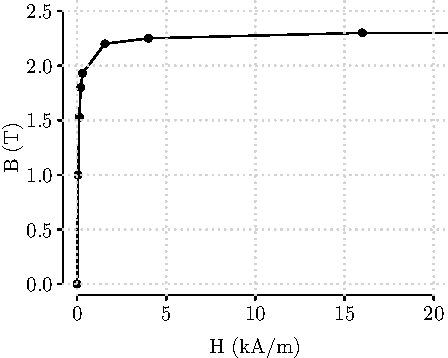
\includegraphics[]{vacoflux_50}
  \caption{B-H curve for  VacoFlux50 cobalt-iron alloy\cite{vacoflux}.}
  \label{vacoflux-bh}
\end{figure}



\section{Electromagnetic Modelling}	
The claw pole machine is modeled using 3D FEA software.

The armature can be built using distributed and concentrated coils.

The machine has two symmetry planes:

\begin{itemize}
	\item Rotational symmetry depending on the number of pole-pairs.
	\item Axial symmetry along the mid-plane passing through the superconducting coil.
\end{itemize}

\section{Optimization}






%Alti ayni
%--------------

\section{HTS Machines}

Superconducting electrical machines have drawn interest since the discovery of the first superconductors in 1911. With high-temperature superconductors and the 2$^{nd}$ generation of HTS wires, research on HTS machines has been boosted. Previous HTS machine topologies are summarized perfectly in \cite{Kalsi2004, Barnes2005,Gieras2008a}. Among these machines, the most common type is a hybrid superconducting synchronous machine with a superconducting dc-field winding in the rotor and non-cryogenic conventional copper armature in the stator \cite{Barnes2005, Klaus2007}. The rotor may include a cold or warm magnetic core or it can be an air-cored rotor. In the latter case, stator teeth can be removed to reduce saturation in the magnetic core, and thus to obtain a higher flux density. The absence of the iron core reduces the synchronous reactance of superconducting machines which will increase the dynamic performance (desirable for wind turbines) and reactive power capability \cite{Kalsi2004}. On the other side, there are some reliability and maintenance issues related to cryocooler coupler and field excitation brushes, which will be addressed in the following section.

In theory, the highest power density can be achieved with a full-superconducting generator. However, in practice superconductors have zero resistance only for dc conditions \cite{Bray2009}, and a superconducting armature winding will experience significant ac losses due to rotating magnetic field \cite{Barnes2005}.  The power of the cryocooler has to be increased to compensate for the extra ac losses. Furthermore, the critical flux density of the superconductor wire decreases significantly in ac conditions \cite{Barnes2005}. For example, Sugimoto \textit{et al.} proposed a 400 kW, 250 rpm axial flux PM machine \cite{Sugimoto2007a} with superconducting armature windings, but due to ac losses they had to use iron cores to divert the magnetic flux from the superconducting coils which will limit the magnitude of magnetic flux density. Without the discovery of a reasonably ac tolerant superconductor wire, full-superconducting machines are not worthwhile, and until that time hybrid superconducting machines will be the workhorse for superconducting machine applications \cite{Barnes2005,Klaus2007}.

Another method is to use magnetized superconducting bulk materials (also known as superconducting magnets). The well-studied property of superconductors showed that, the magnetic flux can be trapped in superconductors through internally circulating super-currents \cite{Bray2009}. It has been reported in \cite{Tomita2003} that magnetic field density up to 17 T can be stored in bulk superconductors.  An axial flux motor for aircraft propulsion with very high power density has been designed using bulk superconducting magnets in \cite{Masson2007, Masson2007b}. In \cite{Matsuzaki2006}, a HTSG with bulk superconductors are designed for ship propulsion applications. If there is no in-situ magnetization system for bulk superconductors, the magnets have to be pre-magnetized and have to be kept at cryogenic temperatures. The enormous magnetic attraction forces makes the assembly process even more challenging than the assembly of large PM machines. Furthermore, the loss of cooling power will result in total demagnetization of HTS magnets. These issues may be overcome by having an in-situ magnetization system within the machine as shown in \cite{Masson2007}. But, the maximum flux density achievable by this systems is quite limited. In \cite{Coombs2009}, a new flux pumping method has been introduced that can magnetize superconductors by repeatedly applying small magnetic flux pulses.  Unless such a method is scaled to larger applications, HTS generators using magnetized superconductors are not feasible for offshore wind turbines.


\subsection{Direct Drive HTS Applications}
In this section, some direct-drive HTSG studies in literature are summarized. One early commercial area for HTS machines was ship propulsion systems. In \cite{Lee2008} a 5 MW, 230 rpm homopolar HTS machine has been presented. The flux density in the air gap varies between 0.9 T and 0.2 T. Also, a comparison between air-cored superconducting synchronous machine(ASSM) and homopolar HTS machine was given; the homopolar machine uses half of the superconductor of ASSM but it is 2.4 times heavier than the ASSM due to the mass of magnetic core. Another propulsion motor is the AMSC's 36.5 MW, 120 rpm  superconducting machine with a rated torque of 2905 kNm, which is expected to be 75 tonnes \cite{Kalsi2004,Snitchler2010}.

Converteam is one of the companies interested in the application of HTSG for offshore wind turbines. They proposed an 8 MW, 12 rpm superconducting generator, which will be 5 m in diameter and approximately 100 tonnes \cite{Lewis2007}. In \cite{Maki2008} a HTSG machine design for a wind turbine is presented with 2, 5, 8 MW options, the masses of the generators have been estimated as 54, 108, 154 tonnes respectively. Snitchler \textit{et al.} have presented an offshore turbine generator design for AMSC Windtec rated at 10 MW, which will have an outer diameter of 4.5-5 m and have a mass of 150 tonnes \cite{Snitchler2010}.

In \cite{Ohsaki2009} a novel generator topology has been presented for wind turbines. In the rotor, superconducting field windings are used to generate dc field, then instead of using ferro-magnetic cores to concentrate the magnetic flux, arc-shaped bulk superconductors are utilized to shield the magnetic flux which results in varying magnetic flux on the armature coils. It is reported that air-gap flux densities between 2.9 T and 0.7 T have been achieved. The design offers high power density but suffers from mechanical issues such as; cryocooler coupler, electrical brushes, and electromagnetic torque acting on superconductors.

\section{Requirements for a HTSG Wind Turbine}
The high efficiency of HTS machines have been emphasized in the first applications. But, efficiency is not solely sufficient.  In order to penetrate into the renewable energy market, HTSG's have to prove that they are also more reliable than alternative power take-off systems such as DDPM machines and geared induction machines \cite{Abrahamsen2010}. Other requirements can be listed as  availability and low-cost.

\subsection{Reliability}
In a HTS machine, the cryogenic system holds the risk of decreasing the overall reliability. In particular, the cryogenic pump and couple are the most critical components. The cryogenic coupler can be eliminated by using a stationary superconducting field, which has many advantages \cite{Gieras2008a};
\begin{itemize}
\item No cryogenic coupler, more robust and cheap cooling system
\item No brushes or complex excitation systems
\item No centrifugal forces and transient torques that can damage the superconducting material
\item Simpler winding support
\end{itemize}

The ac tolerance of superconducting wires are not satisfactory \cite{Bray2009} and has the aforementioned disadvantages. Thus, a dc field winding will be beneficial in the following ways;
\begin{itemize}
\item Maximized current density with perfect conductivity
\item No excess heat is generated, minimized cooling power
\item Minimized possibility of a local quench due to non-homogeneous flux density distribution
\end{itemize}

The windings of conventional generators experience continuous thermal cycles, which reduces the life expectation of the insulation and causes a common type of failure \cite{Gieras2008a,Spinato2009}. However, the field winding of a HTS machine is  maintained at a constant low temperature without any thermal cycles, increasing the reliability of the insulation system. Furthermore, the chemical degradation rate of insulation at cryogenic temperatures is significantly low \cite{Lewis2007}.


\subsection{Availability}

The availability of the generator is a direct factor affecting the electricity generation income. The interval of maintenance should be scheduled starting from the design stage. The present generation of cryocoolers do require periodic    maintenance, for example a cryocooler of a 4.5 MW HTS machine has a maintenance cycle of 10,000 hours \cite{Schiferl2006}. If the generator design dictates turning off the cryocooler, then cooling times, which can be up to several hours, should be considered. For instance, a cold magnetic core is used in \cite{Wen2009} for a 100 kW generator, with a cooling power of 120 W. The generator can be cooled down to operating temperature (67 K) from ambient temperature in 18 hours. Another example is Siemens' 4 MW machine which has a total cooling power of 135 W. The cooling time for this machine is approximately 75 hours \cite{Klaus2006}. In order to increase availability;

\begin{itemize}
\item The cold mass of the generator should be minimized, a warm-iron core is preferable.
\item The cryocooler system should have some redundancy to enable the maintenance while keeping the superconducting coil at cryogenic temperatures.
\end{itemize}

Zenergy and Converteam involved in a research project to work on the development of maintenance-free cryocoolers \cite{Lewis2007}. Snitchler \textit{et al.} described a particular refrigeration system, which has MBFR(mean time between failure rate) longer than 9 years \cite{Snitchler2010}. They also proposed using six to ten cryocoolers with N+1 redundancy with a maintenance cycle of 2 years for cryocoolers, fans and seals.

\subsection{Cost}

The initial cost of the generator is crucial. In \cite{Maples2010}, the cost of HTS machine is estimated to be lower than the cost of geared solutions for greater than 6.5 MW, and 8 MW for direct-drive PM generators. This estimation is based on the current HTS wire prices, but Lewis and M\"{u}ller proposed that the price of  2\textsuperscript{nd} generation HTS wires will beat the current copper prices as demand increases \cite{Lewis2007}. Lesser \textit{et al.} has taken this forecast into account and estimated that the HTS machines will have lower cost than direct-drive PM generators for applications larger than 5 MW \cite{Lesser2009}. The machine topology has a direct effect on the generator cost. But note that, installation costs, availability and efficiency should also be included in calculations to obtain a more reasonable comparison between different type of generators.


\section{Proposed Generator Topology}


In order to find a suitable topology for offshore wind turbines with the said specifications, homopolar HTSG's are chosen as the first candidate. Homopolar machines have several advantages owing to the stationary superconducting field winding \cite{Gieras2008a,Lee2008} many of the which are mentioned in the previous section.  They may be the most reliable HTSG topology but due to large magnetic core requirements and homopolar variation of air gap flux, the power density of presented machines are not very high. More over, homopolar HTSG's in literature are not optimized for very low speed range, i.e. for large diameters. Addressing this shortcoming an axial flux homopolar machine is proposed.

\subsection{Axial Flux Homopolar Superconducting Machine}

The generator is designed for low-speed applications, so it has to have a large diameter to increase the torque capability. The stator composes of an air-cored copper armature winding and a stationary large circular superconducting field winding as given in Fig. \ref{axial_homopolar_stator_rotor}. The armature coils are attached to a fixed outer ring support structure, which can be mounted on the circumference of the nacelle. The superconducting  field winding is a large circular single superconducting coil. The superconducting coil is fixed to the armature coils. There is no electro-magnetic torque acting on the field winding which simplifies the support structure. One challenge may be the manufacturing and assembly of the large diameter, single piece of winding. On the other side, it is believed that a technology transfer from superconducting power transmission cable manufacturing industry is possible, which will reduce the cost of the field winding. The end-side of the field winding can be connected directly to cryocooler and excitation system without using any moving parts as shown in Fig. \ref{axial_homopolar_stator_rotor}.


\begin{figure*}[!h]
\centerline{\subfigure[]{\includegraphics[width=3in]{axial_homopolar_stator_rotor}
\label{axial_homopolar_stator_rotor}}
\hfil
\subfigure[]{\includegraphics[width=3in]{magnetic_pole_dimensions}
\label{axial_homopolar_dimensions}}
}
\caption{ Axial flux homopolar superconducting machine. a) Stator (mechanical structure is not shown) and rotor.
b) Main dimensions of the homopolar magnetic core.}
\end{figure*}

The rotor has a varying reluctance structure with many modular magnetic core sections. For example, the generator presented in in Fig. \ref{axial_homopolar_stator_rotor} composes of 60 modular magnetic cores and 45 concentrated armature coils. The rotor sections are C-shaped and arranged to constitute a disc-shaped translator. The shape of the C-core should be optimized to maintain low weight and uniform flux density distribution. The gaps between cores can be left as air gap or can be filled by any non-magnetic material to increase stiffness of the structure. The magnetic flux generated by the stationary superconducting coil is diverted by these modular ferromagnetic materials, creating a varying flux on the armature coils. Note that, since the armature coils are air-cored there is no magnetic de-centring forces between stator and rotor, which will simplify the manufacturing of support structure. The cut-through view of the machine is presented in Fig. \ref{axial_homopolar_section}. The insulation layer in the superconducting field winding with expected magnetic flux vectors are also shown. The flux density vectors obtained from 3D FEA software in a half-symmetry C-core is given in Fig. \ref{axial_homopolar_flux_vectors}. 

\begin{figure*}[h]
\centerline{\subfigure[]{\includegraphics[height=2in]{axial_homopolar_section}
\label{axial_homopolar_section}}
\hfil
\subfigure[]{\includegraphics[height=2in]{axial_homopolar_flux_vectors}
\label{axial_homopolar_flux_vectors}}
}
\caption{Axial flux homopolar superconducting machine. a) Cut-through view of rotor and stator. b) FEA simulation in half-symmetry C-core, superconducting coil, insulation layer and flux density vectors are shown.}
\end{figure*}

For minimum mass and maximum utilization of the magnetic core, each dimension should be defined correctly. For this purpose, web area, core area and pole tooth area (perpendicular to the direction of magnetic flux) as shown in Fig. \ref{axial_homopolar_dimensions} should be equalized. These terms can be defined respectively as;
\begin{equation}
    A_{web}=\frac{\theta_{pole}}{2}(r_{web}^2-r_{in}^2)
\end{equation}
\begin{equation}
    A_{core}=\theta_{core}r_{tooth}t_{c}
\end{equation}
\begin{equation}
    A_{tooth}=\frac{\theta_{core}}{2}(r_{out}^2-r_{tooth}^2)
    \label{A_tooth}
\end{equation}
where $\theta_{pole}$ is the pole pitch angle, $\theta_{core}$ is the magnetic core pitch angle, $r_{out}$ is the outer radius of rotor, $r_{tooth}$ is the tooth inner radius, $r_{web}$  is the web radius, $r_{in}$ is the inner radius of rotor,  $t_{c}$ is the thickness of core limb. Equalising these areas ensures equal flux densities through the core and allowing the core to be excited up to its saturation limit. The tooth tapering can be adjusted to ensure constant flux density through its span. The magneto-motive force of the superconducting coil can be calculated as;
\begin{equation}
    NI_{sc}=J.A_{winding}.k_{fill}
\end{equation}
where $J$ is the current density, $A_{winding}$ is the winding area and $k_{fill}$ is the fill factor including thermal and electrical insulation. All core sections experience same magnetic potential regardless of position. Identical reluctance of cores create a tangential symmetry i.e., identical resistances are connected in parallel to a constant voltage source. Then core and air gap reluctance of a single section can be defined as;

\begin{equation}
    \Re_{core}=\frac{h_{g}+\pi t_{c}+2(w_{g}h_{t})+\sqrt{t_{c}^2+l_{m}^2}}{A_{core}\mu_{0}\mu_{c}}
\end{equation}

\begin{equation}
    \Re_{gap}=\frac{2a_{c}+h_{w}}{A_{tooth}\mu_{0}}
\end{equation}
where $h_{g}$ is the height of the gap (for field winding), $w_{g}$ is the radial width of the gap (for field winding), $h_{t}$ is the height of tooth, $l_{m}$ is the length of tooth, $A_{core}$ is the core cross-section area, $\mu_{0}$ is the permeability of air, $\mu_{c}$ relative permeability of core, $a_{c}$ is the clearance from tooth to armature coil, $h_{w}$ is the height of the armature winding, $A_{tooth}$ is the axial area of tooth as given in (\ref{A_tooth}).

Although the analytical model gives a good estimation of the magnetic circuit characteristics, the flux density distribution has also been calculated using 3D FEA software; Opera Vector Fields. FEA results give better understanding of fringing and leakage flux from core teeth.  In order to see the effect of fringing flux and to find the optimum core to pole angle ratio ($ \theta_{core} /\theta_{pole}$) different simulations are performed with varying core to pole ratios. The air gap flux density distribution is compared in Fig. \ref{axial_homopolar_flux_density}.

\begin{figure}[!h]
\centering
\includegraphics[width=3in]{axial_homopolar_flux_distribution}
\caption{Air gap flux density distribution with $ \theta_{core}/\theta_{pole}$ ratio from 0.1 to 0.9 for axial flux homopolar machine.}
\label{axial_homopolar_flux_density}
\end{figure}

The maximum value of the air gap flux density is limited by saturation in the core, which is around 1.32 T. The minimum value of the flux density is larger than zero due to said fringing flux. Therefore, even if the maximum flux density is increased up to the maximum saturation limit, the magnetic flux variation is limited, also limiting the induced voltage in the armature coils. The largest difference between the maximum and the minimum flux density values is obtained as 0.77 T for core to pole angle ratios between 0.4--0.5.  It is obvious that, the power density of such a machine will be quite limited due to homopolar variation of the air gap flux density.


\subsection{Axial Flux Bipolar Superconducting Machine}


The homopolar machine presented in the previous section has many mechanical advantages, but its electromagnetic performance is not very satisfactory. The winding arrangement of the homopolar machine can be modified to create two opposing magnetic fields.  For that, two separate superconducting field windings should be used as presented in Fig. \ref{axial_bipolar_stator_rotor}. The inner field winding is fixed to the armature windings similar to the one in homopolar version. The outer field winding is fixed into a magnetic back-core to divert the magnetic flux. Both field windings carry dc current in the same direction. The  magnetic flux created by inner and outer field windings are carried through rotating inner and outer magnetic cores, linking armature coils in $+y$ and $-y$ directions respectively. The cut-through view of the machine and magnetic flux directions are shown in Fig. \ref{axial_bipolar_section}. Note that, these two cores are magnetically separated, however outer cores are mechanically fixed to inner cores with a non-magnetic structural material e.g. aluminium, nickel based steel.

\begin{figure*}[!h]
\centerline{\subfigure[]{\includegraphics[height=2.5in]{axial_bipolar_stator_rotor}
\label{axial_bipolar_stator_rotor}}
\hfil
\subfigure[]{\includegraphics[height=2.5in]{axial_bipolar_section}
\label{axial_bipolar_section}}
}
\caption{Axial flux bipolar superconducting machine. a) Stator and rotor components of the machine. 
b) Cut-through view of the machine. Armature coils, superconductor windings and back core(dark grey) are stationary; rotor structure, inner magnetic core and outer magnetic core(light grey) are rotating. }
\end{figure*}

The flux density distribution in the machine is simulated in 3D using FEA software; Opera Vector Fields. Fig. \ref{axial_bipolar_vectors_air} shows the flux distribution in the core and in the surrounding air. The current density in the field winding area is 100 A/mm$^{2}$. The field winding is covered with a super-insulation layer. The fill factor of the winding is taken as 0.2. The magnetic core also functions as a flux diverter, reducing the amount of flux penetrating into the superconductor material. Fig. \ref{axial_bipolar_vectors_air} shows the magnitude of vertical magnetic flux penetrating into superconducting material is no more than 0.5 T.  Fig. \ref{axial_bipolar_vectors} show the flux density distribution in inner and outer cores. The cores are represented by half symmetry for simplicity. The grey region shows the non-magnetic support structure. The leakage flux paths between facing surfaces of opposite poles can be observed. This leakage flux reduces the amount of flux linking the armature coils and should be minimised.


\begin{figure*}[!h]
\centerline{\subfigure[]{\includegraphics[width=3in]{axial_bipolar_flux_vectors}
\label{axial_bipolar_vectors_air}}
\hfil
\subfigure[]{\includegraphics[width=2.5in]{axial_bipolar_flux_vectors_iso}
\label{axial_bipolar_vectors}}
}
\caption{Axial flux bipolar superconducting machine. a) Flux density vectors on the side surface of the axial flux bipolar superconducting machine, b) Flux density vectors in the axial flux bipolar superconducting machine(half-pole symmetry is applied). }
\end{figure*}


\subsubsection{Magnetic Core Optimization}


In order to find the optimum aspect ratio for magnetic core, various FEA simulations have been performed. Firstly, the distance between adjacent poles ($t_{min}$) has been varied whereas the axial gap between teeth ($g$) and core to pole pitch ratio ($\tau_{core}/\tau_{pole}$) has been kept constant as given in Fig. \ref{varying_tmin_gap_ratio}.  The simulations have been performed for three different core types presented in Fig. \ref{varying_misalign}. The first core has the largest amount of magnetic core which covers the superconducting field winding completely. This core type has a small core reluctance, but it also has a high leakage flux between opposing poles. The flux linkage for each core type has been calculated and compared using 3D FEA results.

\begin{figure*}[!h]
\centerline{\subfigure[]{\includegraphics[width=2in]{varying_tmin_gap_ratio}
\label{varying_tmin_gap_ratio}}
\hfil
%\\
\subfigure[]{\includegraphics[width=2in]{core_types}
\label{core_types}}
\hfil
%\\
\subfigure[]{\includegraphics[width=2in]{varying_misalign}
\label{varying_misalign}}
}
\caption{Optimising aspect ratio of core for bipolar axial flux machine. a) Varying distance between adjacent poles ($t_{min}$) to axial gap between teeth ($g$) ratio, whereas core to pole pitch ratio ($\tau_{core}/\tau_{pole}$) is constant.
b) Different core types; full-core with all magnetic core, half-core with a non-magnetic core support with a pitch of $\tau_{core}$, simple-core with a non-magnetic core support with a pitch of $\tau_{pole}-\tau_{core}$.
c) Varying alignment of poles.}
\end{figure*}

The power densities for different cases can be compared as follows. The magnitude of the induced voltage in a coil with single turn can be expressed as in(\ref{induced_voltage}), where $\nu$ is the linear speed of rotor, $\lambda_{pk}$ is the peak flux linkage, $\tau_{pole}$ is the pole pitch. The total number of coil in the generator can be calculated with (\ref{n_coil}) by assuming coil pitch ($\tau_{coil}$) equals to $\frac{4}{3}\tau_{pole}$, where $R$ is the mean air gap radius. Then, total power output of the generator can be expressed using (\ref{power_out}), where $N_{t}$ is the number of turns per coil, $I_{coil}$ is the coil current. Finally, if the constants are removed from (\ref{power_out}), it can be seen the power is directly proportional with the ratio of peak flux linkage to pole pitch squared as presented in (\ref{p_out}).

\begin{equation}
    e=\dfrac{\pi.\nu.\lambda_{pk}}{\tau_{pole}}
    \label{induced_voltage}
\end{equation}

\begin{equation}
    N_{coil}=\dfrac{3\pi R}{2\tau_{pole}}
    \label{n_coil}
\end{equation}

\begin{equation}
    P_{out}=\dfrac{\pi.\nu.\lambda_{pk}}{\tau_{pole}}N_{t}I_{coil}\dfrac{3\pi R}{2\tau_{pole}}
	\label{power_out}
\end{equation}

\begin{equation}
    P_{out} \propto \dfrac{\lambda_{pk}}{\tau_{pole}^{2}}
    \label{p_out}
\end{equation}

The core types presented in Fig. \ref{core_types} are simulated in 3D FEA software with varying gap between adjacent poles and the results are compared using (\ref{p_out}) in Fig. \ref{tmin_gap_ratio_graph}. The performances of the full-core and half-core are very low for small values of $t_{min}$. For $t_{min}/g$ ratio larger than two, all coils have similar performance. The best performance can be obtained with a simple-core when the distance between adjacent poles is equal to the distance between the teeth surfaces. The simple-core structure holds considerable amount of non-magnetic material as shown in Fig. \ref{core_types}. This part can be manufactured from light materials, such as aluminium profile or durable plastic to reduce the overall mass. 

Secondly, the distance between the opposing cores are increased gradually as shown in Fig. \ref{varying_misalign}. This reduces the leakage flux between cores and increases the flux linkage but it also increases the coil dimensions and hence the copper losses. The different cases have been compared in terms of the ratio of flux linkage to coil area versus total tooth length in Fig. \ref{misalign_graph}. The best option has been selected as the case with 1.8Lm total tooth distance (refer to Fig. \ref{varying_misalign}).

\begin{figure*}[!h]
\centerline{\subfigure[]{\includegraphics[height=1.75in]{core_plot_a}
\label{tmin_gap_ratio_graph}}
\hfil
\subfigure[]{\includegraphics[height=1.75in]{core_plot_b}
\label{misalign_graph}}
}
\caption{a) Flux linkage to pole pitch squared ratio($ \lambda_{peak}/\tau_{pole}^2$) as a function of $ t_{min}/gap $ ratio for different core types.
b) Flux linkage to coil area ratio ($ \lambda_{peak}/A_{coil} $) as a function of displacement of cores.}
\end{figure*}

After defining the optimum aspect ratio for the generator, the flux density distribution on the coil surface is visualized using Opera 3D FEA software in Fig. \ref{flux_density}. From the figure it can be seen that the densities up to $\pm$1.38 T can be achieved in the armature coils. The armature coils are air-cored, therefore saturation in the stator teeth is eliminated. Moreover, there is no magnetic attraction force between rotor and stator, eliminating the normal forces on armature structure and simplifying the mechanical structure design. 


\subsubsection{The Conceptual Design}

After the optimum aspect ratios for the proposed topology is determined, a 6 MW, 12 rpm direct-drive axial-flux bipolar superconducting generator has been designed. The resulting conceptual generator design is 12 m in diameter, and weights approximately 134 tonnes, including 30 tonnes of structural mass. The full specifications of the design are presented in Table \ref{generator_specs}. Rated torque of the generator is 4,775 kNm, which corresponds to a generator mass of 97.5 tonnes, if trend-line equation for HTS generators presented in (\ref{mass_torque_eq}) is applied. Therefore, the proposed design is 40\% heavier than the expected value for HTSG. With a mass to torque ratio of 28 kg/kNm, the proposed generator is slightly heavier than the PM generator equivalent. Although, this mass can be slightly reduced by using a coupled electro-magnetic and structural optimization tool, the generator is expected to have a higher mass due to large magnetic core requirements. 





\begin{figure}[t]
\centering
\includegraphics[width=3in]{flux_density}
\caption{Flux density distribution in the air gap (perpendicular to armature coil surface) with the optimized core type, $t_{min}/g$ ratio, and displacement ratio, shaded area shows the armature coil area.}
\label{flux_density}
\end{figure}


\begin{table*}[h]
\caption{Conceptual Design Specifications}
\label{generator_specs}
\centering
\begin{tabular}{lll}
\hline
\hline
Rated Power & 6 & MW \\
Rated Speed & 12 & RPM \\
Rated Torque & 4,775 & kNm \\
Outer Diameter & 12 & m \\
Number of Poles & 360 \\
Number of Coils & 270 \\
Electrical Frequency & 36 & Hz \\
Efficiency & 94.5 & \% \\
Length of SC Wire & 43 & km\\
Mass of Single Core & 260 & kg \\
Total Mass & 134 & tonnes \\
Torque Density & 28 & kg/kNm \\
\hline
\hline
\end{tabular}
\end{table*}



\section{Conclusion}
This study set out to determine the requirements of a HTSG power take-off system for large offshore wind turbines.  Firstly, diverse number of direct-drive generators have been compared in terms of their torque densities. HTSG generators generally have smaller mass for the same torque requirements, especially for applications that demand more torque than 3000 kNm. Secondly, the necessities for offshore wind turbine power take-off systems have been defined. In contrast to the first HTSG applications where the efficiency was the primary issue, emphasis should be on the reliability of the generator. To answer that, two different topologies have been proposed. The homopolar axial flux HTSG has a very simple structure with its modular core structure and stationary superconducting field winding, but it suffers from single polar distribution of magnetic flux which reduces the induced voltage magnitude. The bipolar axial flux machine can achieve larger flux density variations, but two separate superconducting field windings are needed. For firstly proposed core type, there is considerable amount of leakage flux. It has been shown that by using different types of cores and certain aspect ratios, the amount of leakage flux can be minimized and the power density can be maximized. The optimum aspect ratios are applied on a 6 MW, 12 rpm turbine, the resulting generator is 134 tonnes including the structural mass, which corresponds to a mass to torque ratio of 28 kg/kNm which is slightly larger than a PM generator. The mass can be reduced with a optimization tool that couples structural and cooling issues of the generator. The University of Edinburgh will continue research on an improved and detailed HTSG generator topology that can meet the requirements of the offshore wind energy industry.






% use section* for acknowledgement

%\section*{Acknowledgment}
%The authors would like to thank...





% trigger a \newpage just before the given reference
% number - used to balance the columns on the last page
% adjust value as needed - may need to be readjusted if
% the document is modified later
%\IEEEtriggeratref{8}
% The "triggered" command can be changed if desired:
%\IEEEtriggercmd{\enlargethispage{-5in}}
%\newpage
%\IEEEtriggeratref{25}
% references section

% can use a bibliography generated by BibTeX as a .bbl file
% BibTeX documentation can be easily obtained at:
% http://www.ctan.org/tex-archive/biblio/bibtex/contrib/doc/
% The IEEEtran BibTeX style support page is at:
% http://www.michaelshell.org/tex/ieeetran/bibtex/

% argument is your BibTeX string definitions and bibliography database(s)
%\bibliography{IEEEabrv, C:\Documents and Settings\okeysan\Desktop\My %Dropbox\LaTeX\Ref/Applied_superconductivity_paper}
\bibliography{IEEEabrv,../../LaTeX/Ref/Applied_superconductivity_paper}
\bibliographystyle{IEEEtran}





% that's all folks
\end{document}



